% \begin{figure*}[!tbh]
%     \centering
%     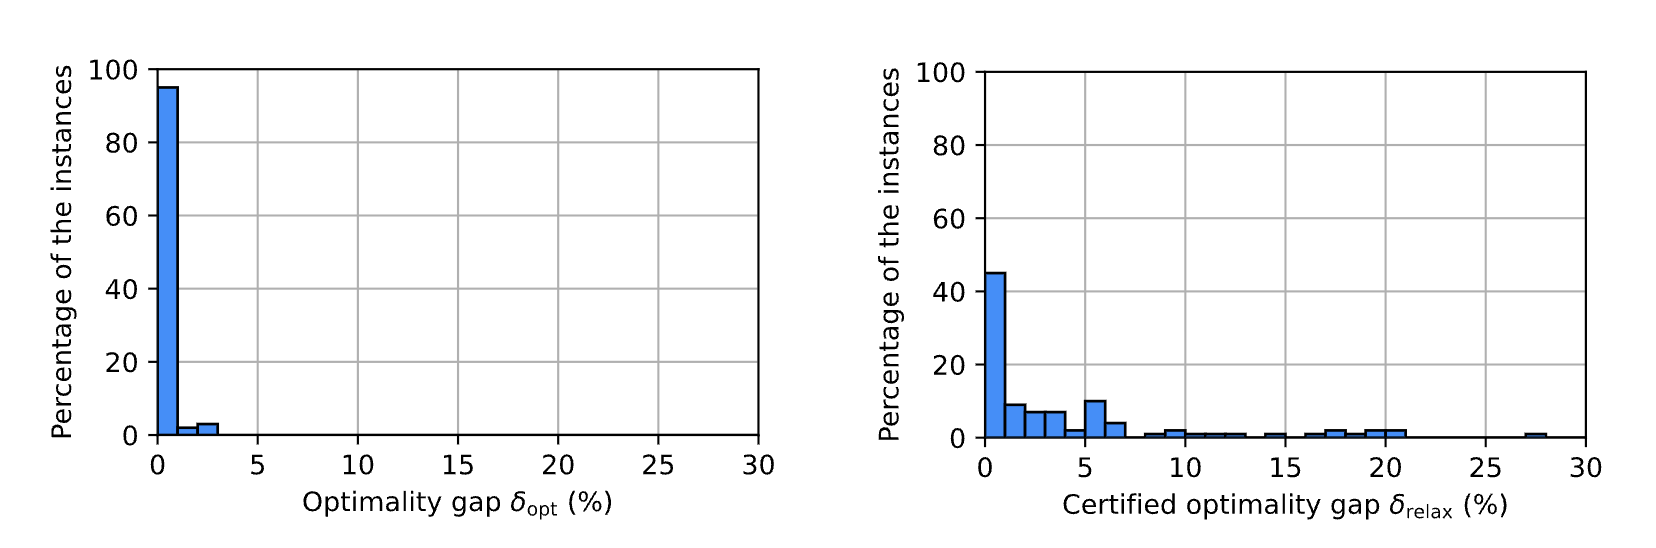
\includegraphics[width=0.8\textwidth]{figures/optimality_gap.png}
%     \captionsetup{justification=centering}
%     \caption{ {\color{red} todo: replace with real figure after running experiments} }
%     \label{fig:}
% \end{figure*}

\begin{figure}[!t]
    \centering
    \begin{subfigure}[b]{0.19\textwidth}
        \centering
        \fbox{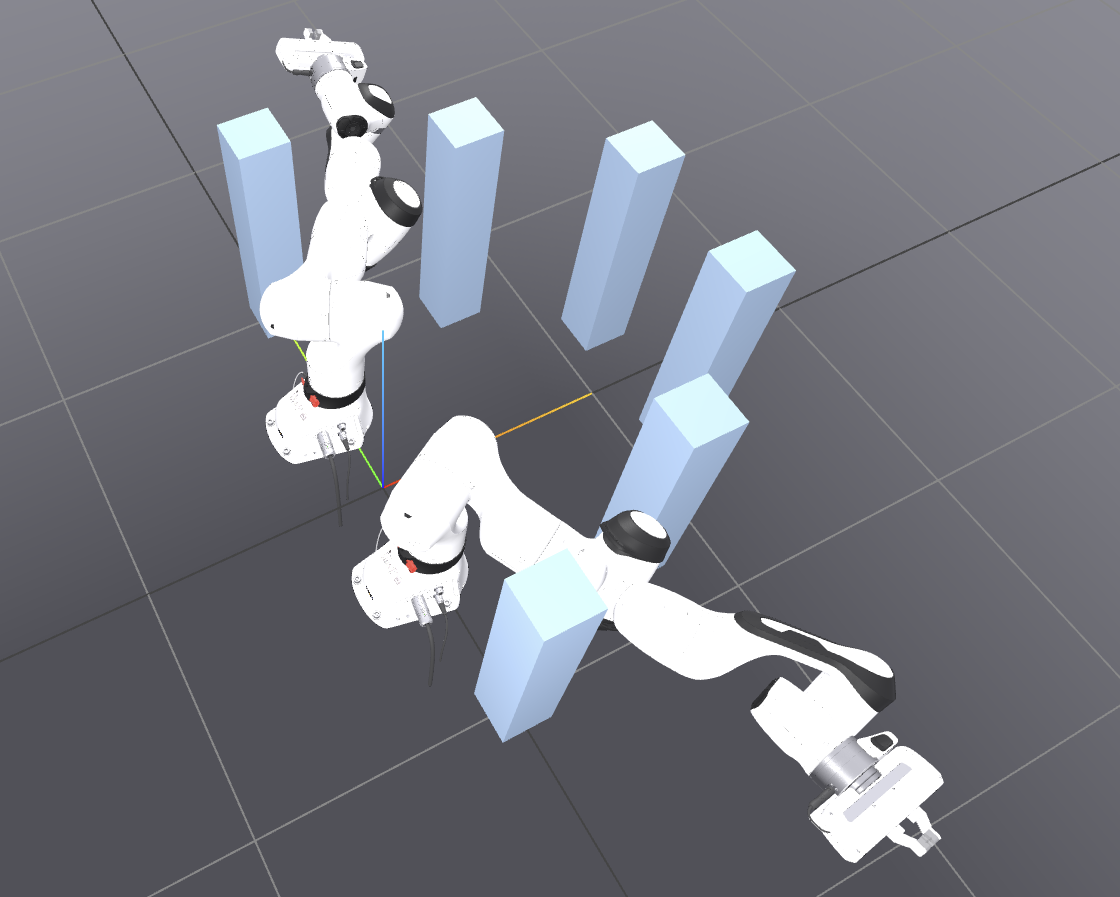
\includegraphics[width=\textwidth]{figures/cage_start_orbit.png}}
        \captionsetup{justification=centering}
        \caption{Start configuration}
        \label{subfig:cage_start_orbit}
    \end{subfigure}\hspace{0.01\textwidth}
    \begin{subfigure}[b]{0.19\textwidth}
        \centering
        \fbox{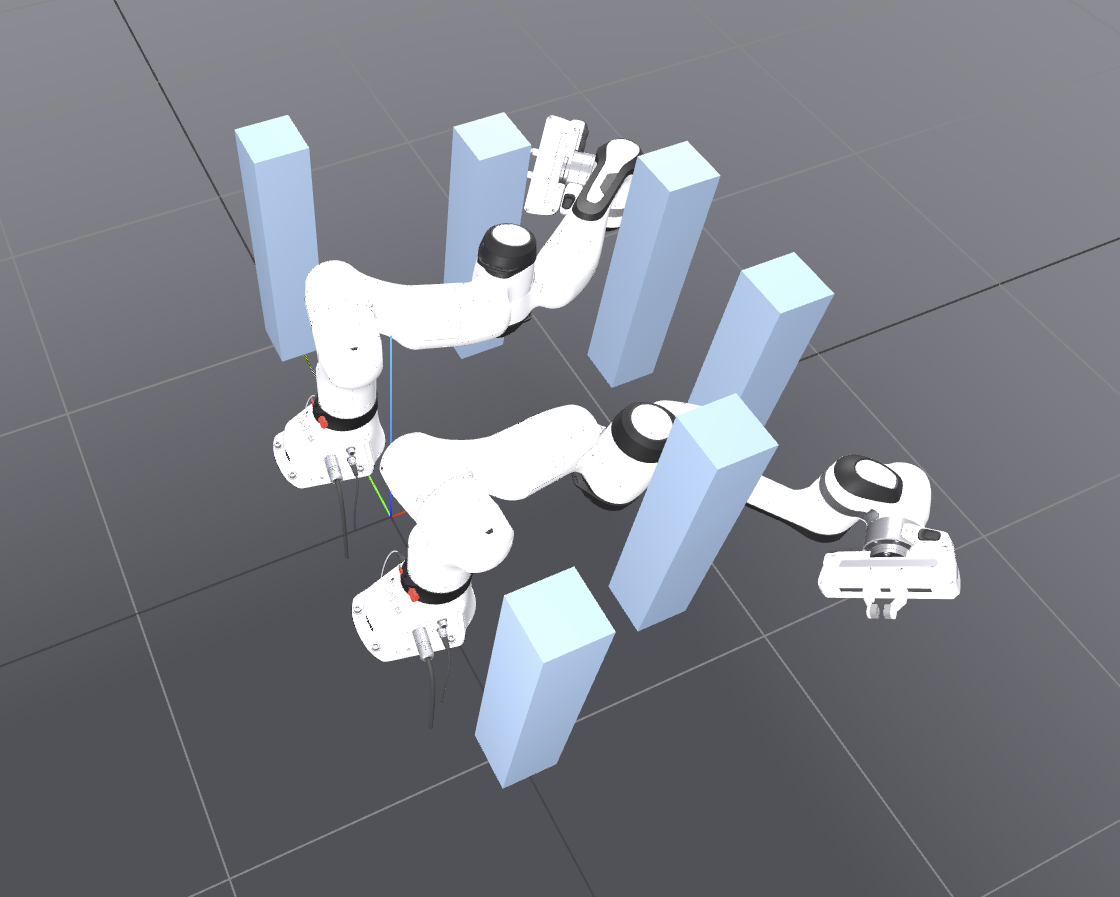
\includegraphics[width=\textwidth]{figures/cage_goal_orbit.png}}
        \captionsetup{justification=centering}
        \caption{Goal configuration}
        \label{subfig:cage_goal_orbit}
    \end{subfigure}
    \caption{A dual-arm manipulation problem for two Franka Emika Panda robots in $\mathbb{R}^{18}$, simulated in Drake. The robots start in an initial configuration (a) positioned between the first two rows of obstacles and must reach the goal configuration (b) between the last two rows of obstacles without collisions.}
    \label{fig:simulation}
\end{figure}

\section{Simulation Results}\label{sec:results}

Our convex optimization-based motion planning approach is primarily built using Drake~\cite{drake}, a widely used toolbox for modeling, simulation and optimization of advanced robotic systems.
We used Drake's implementations of the GCS framework and IRIS to decompose the robot's free configuration space into convex regions.
Note that, to handle the mixed-integer programs generated by the GCS approach, we made use of the MOSEK optimization solver~\cite{mosek}, which supports large scale mixed-integer convex programs.

The robot platform used to validate our approach is a 18-degree-of-freedom dual-arm manipulator as shown in Figure~\ref{fig:simulation}: each robotic arm comprises 7 joints, and its corresponding gripper includes 2 joints.
The environment we designed resembles a cage, where the robot's task is to move from its initial configuration---positioned between the first two rows of obstacles---to a goal configuration located between the last two rows of obstacles.
We purposefully constructed this setup to ensure that narrow passages appear in the high-dimensional configuration space of the robot, a known challenge for classical motion planners.
All aspects of the robot's geometry, kinematics and collisions were modeled using Drake's built in simulation and collision checking engines.

In addition to our approach, we use sampling-based motion planners from the Open Motion Planning Library (OMPL)~\cite{sucan2012open}\footnote{We used the latest release version 1.7.0 of OMPL for all the experiments.} as benchmarks for comparison. All parameters related to these sampling-based planners were carefully reviewed and adjusted only when necessary to ensure a fair comparison. Due to space constraints, detailed configurations are omitted from this report, and interested readers can refer to our publicly available repository for more information.\footnote{\url{https://github.com/utiasSTARS/ece1505-w25-project}}.{\color{red}we should probably move this repo to our own}

% \begin{table}[t]
% \centering
% \caption{GSC results}
% \label{table_1}
% \begin{tabular}{|l|c|c|c|}
% \hline
% Problem size & Small & Medium & Large \\
% \hline
% Relaxation cost & 8.7629 & 8.1071 & 7.4669\\
% \hline
% Rounded cost (min-max) & 8.7629 & 8.1423 & 8.1659\\
% \hline
% Rounded cost (max) & 8.7629 & 8.1423 & 10.0959\\
% % \hline
% % Rounded cost (min-max) & 8.7629-8.7629 & 8.1423-8.1423 & 8.1659-10.0959\\
% \hline
% Rounded cost (average) & 8.7629 & 8.1423 & 8.6566\\
% \hline
% Optimality gap (min) & 0 & 0.0043 & 0.0936\\
% \hline
% Optimality gap (max) & 0 & 0.0043 & 0.3521\\
% \hline
% Optimality gap (average) & 0 & 0.0043 & 0.1593\\
% \hline
% \end{tabular}
% \end{table}

\begin{table}[t]
\centering
\caption{Summary of GCS results for different problem sizes.}
\label{table_1}
\begin{tabular}{lccc}
\toprule
\textbf{Metric} & \textbf{Small} & \textbf{Medium} & \textbf{Large} \\
\midrule
Relaxation cost               & 8.7629 & 8.1071 & 7.4669 \\
Rounded cost (min)            & 8.7629 & 8.1423 & 8.1423 \\
Rounded cost (max)            & 8.7629 & 8.1423 & 11.0726 \\
Rounded cost (average)        & 8.7629 & 8.1423 & 8.7158 \\
\midrule
Optimality gap (min)          & 0.0000 & 0.0043 & 0.0904 \\
Optimality gap (max)          & 0.0000 & 0.0043 & 0.4829 \\
Optimality gap (average)      & 0.0000 & 0.0043 & 0.1673 \\
\bottomrule
\end{tabular}
\end{table}

\subsection{Analysis of the minimum-length trajectory problem}
We tested a version of GCS that minimizes the Euclidean length of the trajectory on graphs of three different sizes: $6$, $12$, and $18$ vertices (see Appendix~\ref{IRIS_details} for more details). Each larger graph contains all the vertices of the smaller ones, along with additional vertices. While it may seem counterintuitive, a larger graph—with more possible configurations—does not necessarily lead to a better (i.e., lower) objective value. For the smallest graph, the feasible objective value after the rounding step is $8.76$; for the medium graph, it is $8.14$; and for the largest, it is $8.66$ (see Table~\ref{table_1}) .

This discrepancy arises from the relaxation used in the problem formulation and the need to apply a rounding step to convert the relaxed solution into a feasible one. Since we employed a randomized rounding method (specifically, a randomized depth-first search with backtracking), we conducted $30$ experiments for each graph size to evaluate performance. To interpret the table results correctly, it is important to note that the optimality gap is evaluated only with respect to the chosen convex sets. Thus, zero optimality gap only means that the solution is optimal with respect to the given graph. For example, although the optimality gap for the smallest graph appears to be zero, the true optimal cost may actually be lower than the obtained solution, since the IRIS convex sets only approximate the full solution space.

As expected, the relaxation cost is the lowest for the largest graph, this is due to the greater number of possible robot configurations. The relaxation is tight for the smallest graph. In the medium-size graph, the relaxation is not tight, but interestingly, the outcome after rounding remains constant across all $30$ experiments. The most variability is observed with the largest graph: although its relaxation cost is the lowest, the rounded cost never outperforms that of the medium graph. Furthermore, the rounded cost in the largest graph varies significantly between experiments, sometimes greatly increasing the initially small relaxation cost.

Additionally, it is important to note that increasing the graph size leads to a significant increase in computation time: GCS takes approximately 0.52 seconds to solve for the smallest graph, 9.89 seconds for the medium graph, and 33.64 seconds for the largest graph (see Figure \ref{fig:exp-b}). Thus, the GCS approach has a scalability limitation, at least when using for highly cluttered environments.

% GCS analysis here
% GCS_6
% Average len: 8.76294017592158
% Average time: 0.6970518021662429

% GCS_12
% Average len: 8.142282537404691
% Average time: 12.900373252932816

% GCS_18
% Average len: 8.6566461563272
% Average time: 51.138213157798845

\begin{figure}[!t]
    \centering
    \begin{subfigure}[b]{\linewidth}
        \centering
        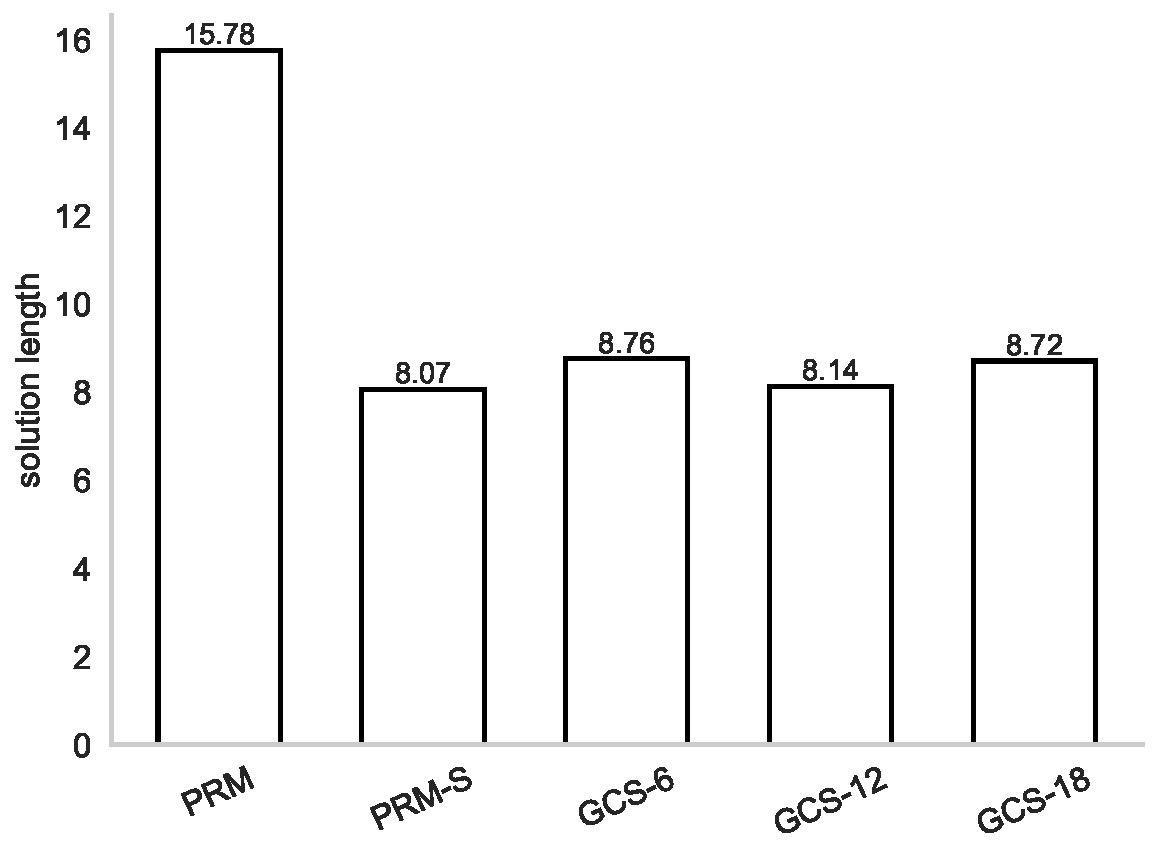
\includegraphics[width=0.85\textwidth]{figures/solution_length_barplot.pdf}
        \captionsetup{justification=centering}
        \label{subfig:}
    \end{subfigure}
    \begin{subfigure}[b]{\linewidth}
        \centering
        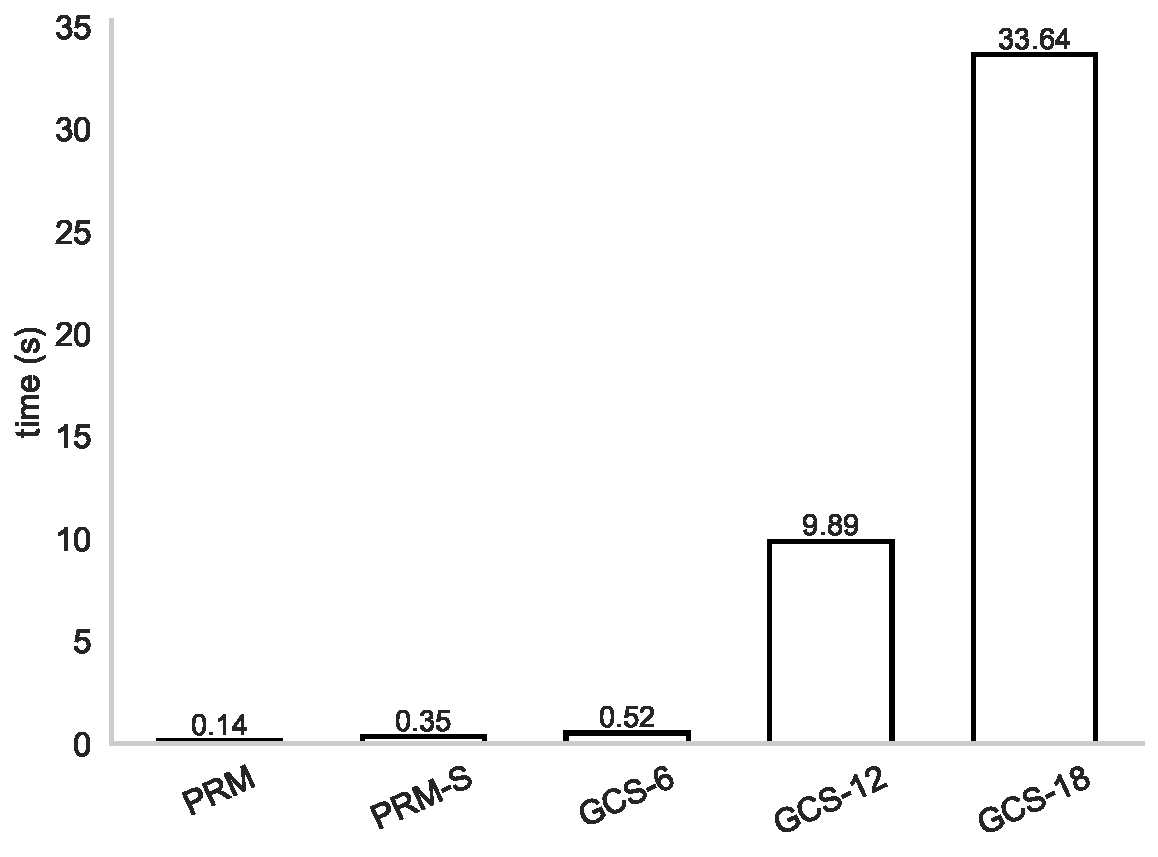
\includegraphics[width=0.85\textwidth]{figures/time_barplot.pdf}
        \captionsetup{justification=centering}
        \label{subfig:}
    \end{subfigure}
    \caption{Average comparison results of the tested algorithms for the dual-arm manipulation problem. The top figure shows the solution quality (measured by path length) across 30 trials for each algorithm. The bottom figure presents the corresponding execution times.}
    \label{fig:exp-b}
\end{figure}

\subsection{Comparison with sampling-based planners}\label{sec:sampling-based}

We also conducted experiments to compare our approach with sampling-based methods, which are standard algorithms used in many high-dimensional motion planning applications. The most suitable candidate for benchmarking against ours is the multi-query sampling-based planner, PRM, as it supports precomputation---these planners build a roadmap (graph) prior to planning to accelerate the solution search. Additionally, we applied path shortcutting techniques to the solution paths found by PRM to improve path quality, with some tradeoff in execution time. Specifically, we used the path shortening method proposed in the work of RRT-Rope~\cite{petit2021rrt}. Each algorithm was run for $30$ trials, and we measured the median solution quality (in terms of path length) and computation time. The results are presented in Figure~\ref{fig:exp-b}. Here, PRM-S denotes PRM with path shortcutting enabled, while GCS-6, GCS-12, and GCS-18 represent our approach using small, medium, and large convex set sizes of $6$, $12$, and $18$, respectively.

In terms of solution quality, we observed that PRM performs the worst among all tested algorithms. This result is also expected, given the known limitations of random sampling-based methods. In contrast, PRM-S and all GCS variants with different set sizes produce comparable solution qualities. Notably, PRM-S achieves the best solution cost among the tested methods, including ours. This represents a significant improvement over the results presented in~\cite{marcucci2023motion}, and demonstrates that our convex optimization-based approach can still compete with state-of-the-art path shortening techniques in terms of solution quality. We also observed that GCS-12 outperforms the other two GCS variants, raising an important question about how to design these collision-free sets and determine their optimal number to strike a balance between performance and computation requirements.

On the other hand, PRM found solutions fastest, with an average computation time of approximately $140$ ms, followed by PRM-S at $350$ ms and GCS-6 at $520$ ms. GCS-12 and GCS-18 took significantly longer, requiring between $9.89$ and $33.64$ seconds to find a solution. These results highlight the importance of selecting an appropriate number and size of convex sets to effectively trade off between solution quality and execution time.

\subsection{Analysis of the extension of the problem}
First, it is important to note that the extended version of Graph-Constrained Search (GCS) runs slower than the version that only optimizes trajectory length. For a graph with six vertices, the extended version is approximately twice as slow. This is due to the use of Bézier curves, which increase the number of configurations optimized at each vertex.

However, this extension provides capabilities not available in traditional sampling-based methods: it allows for control over the smoothness, differentiability, and time optimality of the trajectory. The extended optimization problem introduces three tunable weights: (a) trajectory duration, (b) trajectory length, and (c) the energy of the time derivative of the trajectory. In addition, it is possible to enforce a constraint on the required degree of trajectory differentiability.

We experimented with different combinations of the weights \( a \), \( b \), and \( c \), while ensuring the resulting trajectory was continuously differentiable (once). Although the optimization occurs in configuration space, the resulting end-effector trajectories, that we visualize, exhibit clear differences depending on the chosen weights.

\begin{itemize}
    \item Prioritizing \( a \) results in a high-velocity trajectory with minimal sharp turns.
    \item Prioritizing \( b \) yields a shorter trajectory with sharper direction changes, making it more difficult to follow quickly.
    \item Prioritizing \( c \) produces a very smooth but slower trajectory.
\end{itemize}

% \begin{table}[t]
% \centering
% \caption{Summary of GCS results for different weights.}
% \label{table_2}
% \begin{tabular}{ccc}
% \toprule
% \textbf{a} & \textbf{b} & \textbf{c} \\
% \midrule
% 1 & 0 & 0 \\
% 0 & 1 & 0 \\
% 0 & 0 & 1 \\
% \midrule
% 1 & 1 & 0 \\
% 1 & 0 & 1 \\
% 0 & 1 & 1 \\
% \midrule
% 1 & 1 & 1 \\
% \bottomrule
% \end{tabular}
% \end{table}